\documentclass[10pt]{article}
\usepackage[letterpaper,text={6.5in,8.7in},centering]{geometry}
\usepackage{epic,eepic}
\usepackage{amssymb,amsmath,times,subfigure,graphicx,theorem,tikz,eepic}
%\usepackage{amssymb,amsmath,times,url,subfigure,graphicx,theorem,alltt,eepic,tikz}

%\usepackage{warmread}
%\usepackage[all,import]{xy}
%\usepackage{eepic}

\newcommand{\norm}[1]{\ensuremath{\left\| #1 \right\|}}
\newcommand{\abs}[1]{\ensuremath{\left| #1 \right|}}
\newcommand{\bracket}[1]{\ensuremath{\left[ #1 \right]}}
\newcommand{\braces}[1]{\ensuremath{\left\{ #1 \right\}}}
\newcommand{\parenth}[1]{\ensuremath{\left( #1 \right)}}
\newcommand{\ip}[1]{\ensuremath{\langle #1 \rangle}}
\newcommand{\refeqn}[1]{(\ref{eqn:#1})}
\newcommand{\reffig}[1]{Fig. \ref{fig:#1}}
\newcommand{\tr}[1]{\mbox{tr}\ensuremath{\negthickspace\bracket{#1}}}
\newcommand{\deriv}[2]{\ensuremath{\frac{\partial #1}{\partial #2}}}
\newcommand{\SO}{\ensuremath{\mathrm{SO(3)}}}
\newcommand{\T}{\ensuremath{\mathrm{T}}}
\newcommand{\so}{\ensuremath{\mathfrak{so}(3)}}
\newcommand{\SE}{\ensuremath{\mathrm{SE(3)}}}
\newcommand{\se}{\ensuremath{\mathfrak{se}(3)}}
\renewcommand{\Re}{\ensuremath{\mathbb{R}}}
\renewcommand{\S}{\ensuremath{\mathbb{S}}}
\newcommand{\aSE}[2]{\ensuremath{\begin{bmatrix}#1&#2\\0&1\end{bmatrix}}}
\newcommand{\ase}[2]{\ensuremath{\begin{bmatrix}#1&#2\\0&0\end{bmatrix}}}
\newcommand{\D}{\ensuremath{\mathbf{D}}}
\newcommand{\pair}[1]{\ensuremath{\left\langle #1 \right\rangle}}
\newcommand{\met}[1]{\ensuremath{\langle\!\langle #1 \rangle\!\rangle}}
\newcommand{\Ad}{\ensuremath{\mathrm{Ad}}}
\newcommand{\ad}{\ensuremath{\mathrm{ad}}}
\newcommand{\g}{\ensuremath{\mathfrak{g}}}

\renewcommand{\baselinestretch}{1.2}
\date{}

\renewcommand{\thesubsection}{\arabic{subsection}. }
\renewcommand{\thesubsubsection}{\arabic{subsection}.\arabic{subsubsection} }

\theoremstyle{plain}\theorembodyfont{\normalfont}
\newtheorem{prob}{Problem}[section]
%\renewcommand{\theprob}{\arabic{section}.\arabic{prob}}
\renewcommand{\theprob}{\arabic{prob}}

\newenvironment{subprob}%
{\renewcommand{\theenumi}{\alph{enumi}}\renewcommand{\labelenumi}{(\theenumi)}\begin{enumerate}}%
{\end{enumerate}}%

\newcommand*\circled[1]{%
  \tikz[baseline=(C.base)]\node[draw,circle,inner sep=0.5pt](C) {#1};\!
}


\begin{document}

\vspace*{1cm}

\pagestyle{empty}
\centerline{\LARGE{ MAE3145: Final Exam}}
\vspace*{0.5cm}
\centerline{\Large December 14, 2016}%\\%\vspace*{0.5cm}

\vspace*{6cm}

\centerline{
\begin{tabular}{lll}
\hspace*{5cm}, & \hspace*{5cm}. & \hspace*{4cm}\\\hline
Last Name & First Name & Student ID
\end{tabular}}

\vspace*{6cm}

\centerline{
\begin{tabular}{|c|c|c|c|c|c|c|}\hline
Prob. 1 & Prob. 2 & Prob. 3 & Prob. 4 & Prob. 5 & Total \\
(20) & (15) & (20) & (15) & (10) & (80)\\ \hline
\hspace*{2.cm} & \hspace*{2.cm} & \hspace*{2.cm} & \hspace*{2.cm} & \hspace*{2.cm} & \hspace*{2.2cm} \\
&&&&&\\
&&&&&\\\hline
\end{tabular}}

\renewcommand{\thepage}{\arabic{page}/8}
\clearpage\newpage\setcounter{page}{1}\pagestyle{plain}

\renewcommand{\theprob}{\arabic{prob} \textit{(20pt)}}
\begin{prob}
Mark whether each statement written in \textit{italic font} is True or False.% (for (a)-(d)), or answer the question shortly (for (e)).

\begin{subprob}
%\item \textit{The orbital period of the Mars is greater than the orbital period of the Saturn}. [True, False]
%\vspace*{1.2cm}

\item The orbital radius of the Earth is $149.6\times 10^6\,\mathrm{km}$, and the orbital radius of the Jupiter is $778.6\times 10^6\,\mathrm{km}$. \textit{The standard Hohmann transfer from the Earth to the Jupiter is always more efficient that the bi-elliptic Hohmann transfer between them.} [True, False]

\item Spacecraft $A$ and $B$ are on the same orbit. The chaser spacecraft $A$ executes a phasing maneuver to catch the target spacecraft $B$ after one revolution at the point $A$. \textit{Then, the chaser spacecraft $A$ should increase its velocity at the beginning of the phasing maneuver.} [True, False] 

\centerline{
\setlength{\unitlength}{2.5em}\centering
\begin{picture}(6,5)(-3,-2.5)
\put(1.5,0){\circle*{0.6}}
\put(0,0){\ellipse{5.0}{4.0}}
\put(2.28,-0.816){\circle*{0.12}}
\put(2.5,0){\circle*{0.12}}
\put(2.7,-0.1){$A$}
\put(2.5,-1.0){$B$}
\put(0,2){\vector(-1,0){0.0}}
\put(0,-2){\vector(1,0){0.0}}
\end{picture}}


%\item We wish to transfer a spacecraft from the inner elliptic orbit to the outer elliptic orbit using a Hohmann transfer. \textit{The Hohmann transfer from $A$ to $B$ is more efficient than the Hohmann transfer from $A'$ to $B'$.} [True, False]
%
%\centerline{
%\setlength{\unitlength}{2.5em}\centering
%\begin{picture}(6,5.5)(-3.0,-3)
%\put(1.5,0){\circle*{0.6}}
%\put(-0.5,0){\ellipse{7.0}{4.0}}
%\put(0.5,0){\ellipse{4.0}{2.4}}
%\put(2.5,0){\circle*{0.12}}
%\put(-1.5,0){\circle*{0.12}}
%\put(3,0){\circle*{0.12}}
%\put(-4,0){\circle*{0.12}}
%\put(2.5,-0.3){$A$}
%\put(-4.5,-0.3){$B$}
%\put(-2.1,-0.3){$A'$}
%\put(3.1,-0.3){$B'$}
%\put(-0.5,2){\vector(-1,0){0.0}}
%\put(-0.5,-2){\vector(1,0){0.0}}
%\put(0.5,1.2){\vector(-1,0){0.0}}
%\put(0.5,-1.2){\vector(1,0){0.0}}
%\end{picture}}


%\item A spacecraft is on an elliptic orbit. When it passes through the periapsis $P$, its rocket is fired along the outward radial direction as shown below. Then, \textit{the eccentricity vector $\vec e$ rotates clockwise}. [True, False]
%
%\centerline{
%\setlength{\unitlength}{2.5em}\centering
%\begin{picture}(6,4.5)(-3,-2.5)
%\put(1.5,0){\circle*{0.6}}
%\put(-0.4,0){\ellipse{6.0}{3.0}}
%\put(2.6,0){\circle*{0.12}}
%\put(2.6,0){\vector(1,0){1.2}}
%\put(2.7,-0.4){$P$}
%\put(-0.4,1.5){\vector(-1,0){0.0}}
%\put(-0.4,-1.5){\vector(1,0){0.0}}
%\end{picture}}
%
%
%
%\item A spacecraft is on a circular orbit around the Earth. \textit{Escaping from the Earth gravitational field completely requires a larger velocity increment than rotating its orbital plane by $30^\circ$ without changing the orbital shape and size}. [True, False]
%
%%
%%\item The ground tracks for two spacecraft are illustrated as follows. \textit{The inclination of Spacecraft 1 is greater than Spacecraft 2, i.e. $i_1> i_2$}. [True, False]
%%
%%\centerline{
%%\setlength{\unitlength}{0.1\textwidth}\centering
%%\begin{picture}(6,3.2)(0,0)\footnotesize
%%\put(0,0){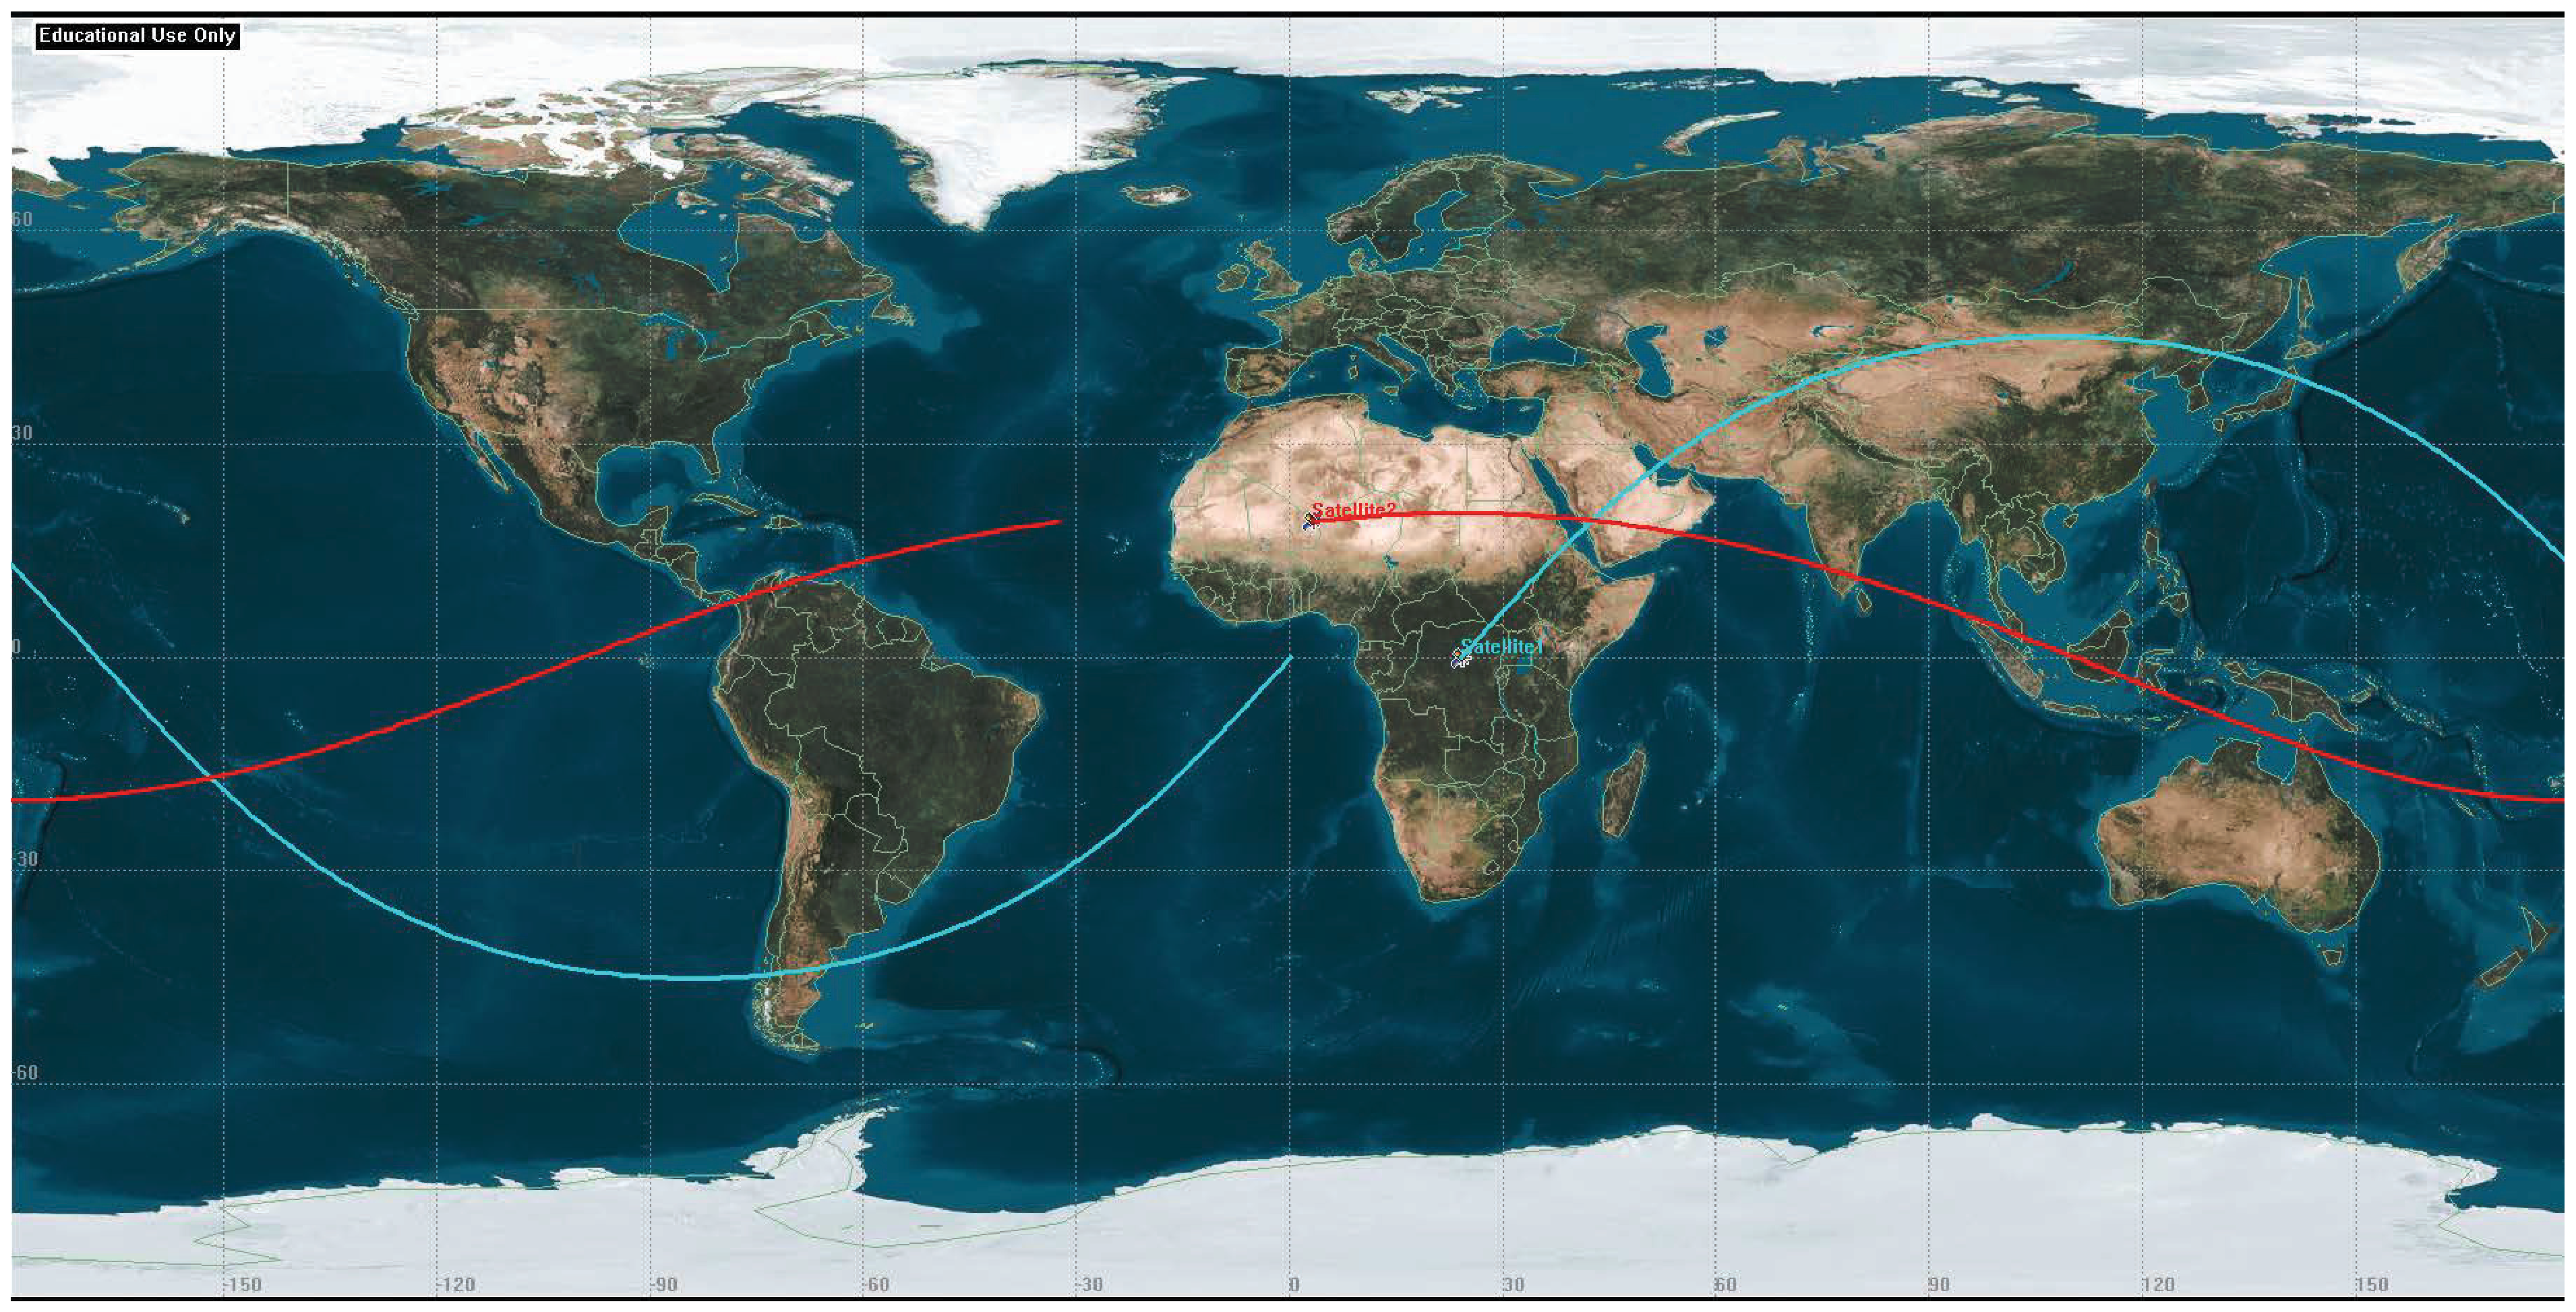
\includegraphics[width=0.6\textwidth]{Prob1.eps}}
%%\put(6.1,1.7){Spacecraft 1 (blue)}
%%\put(6.1,1.05){Spacecraft 2 (red)}
%%\end{picture}}
%
%
%\item \textit{Among the five Lagrange points in the Earth-Moon system, the first Lagrange point $L_1$ has the lowest value of the Jacobi constant, i.e. $L_1$ has the minimum energy.} [True, False]
%
%\item Kennedy Space Center has been NASA's primary launch center of human spaceflight since December 1968. Describe \textit{shortly} one of the \textit{engineering} benefits of locating a lauch center in the southern east coast, compared with other places like Portland, OR. (Please, exclude political or climate-related issues.)


%\item \textit{Among the five Lagrange points in the Earth-Moon system, the first Lagrange point $L_1$ has the lowest value of the Jacobi constant, i.e. $L_1$ has the minimum energy.} [True, False]

\item Consider a satellite on a circular orbit around the Earth. \textit{Changing the orbital inclination by $15^\circ$ requires more $\Delta v$ than that to make it completely escape from the Earth gravitational field.} [True, False] 


\item Consider the circular restricted three body problem for the Earth-Moon system. Let $C_i$ be the value of the Jacobi constant at the $i$-th Lagrange points for $i\in\{1,2,\ldots 5\}$. Suppose that a spacecraft is on a near-Earth orbit, and its Jacobi constant $C$ satisfies $C<C_1$. \textit{This spacecraft has an enough energy to be transferred to the Moon without firing a rocket}. [True, False] 


\end{subprob}
\end{prob}


\begin{prob}

\end{prob}


%\clearpage\newpage

%\begin{prob}
%A spacecraft is on a circular orbit with orbital velocity $v_\circ$. 

%\begin{subprob}
%\item Show that the velocity change $\Delta v_h$ required to transfer the spacecraft into a hyperbolic orbit with eccentricity $e$ is given by
%\begin{align*}
%\Delta v_{h} = v_{\circ} (\sqrt{1+e} -1).
%\end{align*}
%\vspace*{6cm}
%\item 
%\end{subprob}

%\end{prob}


\clearpage\newpage
\renewcommand{\theprob}{\arabic{prob} \textit{(15pt)}}
\begin{prob}
Spacecraft $A$ is on a circular orbit \circled{1} around the Earth, and Spacecraft $B$ is on an elliptic orbit \circled{2} around the Earth.

\centerline{
\setlength{\unitlength}{2.5em}\centering\small
\begin{picture}(5.33,5)(-4.0,-2.0)
\put(-1.0667,0){\ellipse{5.333}{4.888}}
\put(0,0){\circle*{0.8}}
\put(0,0){\circle{3.2}}
\put(-1.7598,0){\circle*{0.1}}
\put(1.6,0){\circle*{0.1}}
\put(-3.733,0){\circle*{0.1}}
\put(1.7,-0.3){$A$}
\put(-4.2,-0.3){$B$}
\put(-2.2,-0.3){$C$}
\put(0,1.6){\vector(-1,0){0.0}}
\put(-1.0667,-2.444){\vector(1,0){0.0}}
\put(-1.2,-1.0){\circled{1}}
\put(-1.8,-1.3){\circled{3}}
\put(-3.7,-1.7){\circled{2}}
\put(-0.08,0){\ellipse{3.3598}{3.356}}
\put(0,0){\line(1,0){1.6}}
\put(0.8,-0.3){$r_A$}
\end{picture}}
\begin{align*}
\mu = 398600\,\mathrm{km^3/s^2},\qquad r_A=8000\,\mathrm{km},\qquad e_2 = 0.4.
\end{align*}

\noindent We wish to design a phase maneuver of Spacecraft $A$ such that rendezvous between Spacecraft $A$ and $B$ occurs at the point $A$ after one revolution. After the rendezvous, Spacecraft $A$ is transferred to Orbit \circled{2}. Let Orbit \circled{3} be the phasing orbit of Spacecraft $A$, and let $C$ be the apoapsis of Orbit \circled{3}.

\begin{subprob}
\item Find the time $t_{BA}$ for Spacecraft B to return to the point $A$.
\vspace*{6cm}
\item Find the period $T_3$ and the apoapsis distance $r_C$ of the phasing orbit \circled{3}.
\newpage
\item Find the velocity change $\Delta v_A = v_{A_3}-v_{A_1}$ at the beginning of the phasing maneuver.
\vspace*{6cm}
\item Find the velocity change $\Delta v_{A'} = v_{A_2}-v_{A_3}$ at the end of the phasing maneuver.
\vspace*{6cm}
\item Show that the total velocity change to complete the phasing maneuver is $1.2933\,\mathrm{km/s}$.

\end{subprob} 
 
\end{prob}





\clearpage\newpage
\renewcommand{\theprob}{\arabic{prob} \textit{(20pt)}}
\begin{prob}
Consider a spacecraft on a circular orbit with radius $r_P$. We wish to rotate the orbital plane by $\delta$ without changing the orbit shape and size. In the class, we found that the required velocity change for one-impulse plane change maneuver is given by
\begin{align}
\Delta v = 2v\sin\frac{\delta}{2},\qquad \text{where }\quad v=\sqrt{\frac{\mu}{r_P}}.\label{eqn:delVoim}
\end{align}
This cost of a plane change is quite high. In this question, we try to reduce the cost of a plane change by designing a series of maneuvers. Let the initial circular orbit be denoted by \circled{1}, and the terminal rotated circular orbit be \circled{4}. The proposed maneuver from \circled{1} to \circled{4} is composed of the following three steps:

\begin{list}{$-$}{\setlength{\itemsep}{0pt}}
\item \circled{1}$\rightarrow$\circled{2} at $P$: transfer the spacecraft to an elliptic orbit \circled{2},
\item \circled{2}$\rightarrow$\circled{3} at $A$: perform a plane change maneuver at the apoapsis $A$ of the elliptic orbit \circled{2},
%\item \circled{2}$\rightarrow$\circled{3} at $A$: transfer the spacecraft back to the periapsis $P$ on the rotated elliptic orbit \circled{3},
\item \circled{3}$\rightarrow$\circled{4} at $P$: transfer the spacecraft to the rotated circular orbit \circled{4} at the periapsis $P$.
\end{list}
Let the apoapsis distance of the transferring elliptic orbits be $r_A>r_P$. These orbits are illustrated as follows:

\centerline{
\setlength{\unitlength}{2.5em}\centering\small
\begin{picture}(6,5)(-3,-2.5)
\put(1.5,0){\circle{2.0}}
\put(1.5,0){\circle*{0.6}}
\put(0,0){\ellipse{5.0}{4.0}}
\put(2.5,0){\circle*{0.12}}
\put(-2.5,0){\circle*{0.12}}
\put(2.7,-0.3){$P$}
\put(-2.9,-0.3){$A$}
\put(0,2){\vector(-1,0){0.0}}
\put(1.5,1){\vector(-1,0){0.0}}
\put(0.45,0.85){\circled{1}}
\put(-2.1,1.6){\circled{2}}
\put(-2.5,0){\line(1,0){5}}
\put(-0.7,-0.3){$r_A$}
\put(1.95,-0.3){$r_P$}
\put(-1.4,-2.5){Initial orbital plane}
\path(-3.2,-2.7)(3.2,-2.7)(3.2,2.3)(-3.2,2.3)(-3.2,-2.7)
\end{picture}
\begin{picture}(4.5,5)(-2,-2.5)
\put(0,0){$\Longrightarrow$}
\put(-0.7,-1.2){\shortstack[c]{plane change\\ maneuver at $A$\\ by $\delta$}}
\end{picture}
\begin{picture}(6,5)(-3,-2.5)
\put(1.5,0){\circle{2.0}}
\put(1.5,0){\circle*{0.6}}
\put(0,0){\ellipse{5.0}{4.0}}
\put(2.5,0){\circle*{0.12}}
\put(-2.5,0){\circle*{0.12}}
\put(2.7,-0.3){$P$}
\put(-2.9,-0.3){$A$}
\put(0,-2){\vector(1,0){0.0}}
\put(1.5,-1){\vector(1,0){0.0}}
\put(0.25,-0.85){\circled{4}}
\put(-2.3,-1.6){\circled{3}}
\put(-2.5,0){\line(1,0){5}}
\put(-0.7,-0.3){$r_A$}
\put(1.95,-0.3){$r_P$}
\put(-2.4,-2.5){Terminal orbital plane, rotated by $\delta$}
\path(-3.4,-2.7)(2.9,-2.7)(3.4,2.3)(-2.9,2.3)(-3.4,-2.7)
\end{picture}
}

\begin{center}\vspace*{0.1cm}
{\small\selectfont
\begin{tabular}{|c|c|c|c|c|c|c|c|}\hline
& Description  & Inclination & Periapsis & Apoapsis & Velocity at the beginning & Velocity at the end\\\hline
Orbit \circled{1} & Initial circular orbit & 0 & $r_P$ & $r_P$ & $V_{P_1}$ & - \\
Orbit \circled{2} & Hohmann transfer orbit & 0 & $r_P$ & $r_A$ & $V_{P_2}$ & $V_{A_2}$ \\
Orbit \circled{3} & Hohmann transfer orbit & $\delta$ & $r_P$ & $r_A$ & $V_{A_3}$ & $V_{P_3}$ \\
Orbit \circled{4} & Target circular orbit & $\delta$ & $r_P$ & $r_P$ & $V_{P_4}$ & - \\\hline
\end{tabular}}
\end{center}

\begin{subprob}
\item Find $\Delta v_P$ to transfer the spacecraft from the initial circular orbit \circled{1} to the  elliptic orbit \circled{2} at $P$.
\vspace*{3.5cm}

\item Find $\Delta v_A$ required to rotate the orbital plane of Orbit \circled{2} by $\delta$ at $A$, transferring the spacecraft to Orbit \circled{3}.
\vspace*{3.5cm}

\item Find $\Delta v_{P'}$ to transfer the spacecraft from the  elliptic orbit \circled{3} to the terminal circular orbit \circled{4} at $P$.
\vspace*{3cm}

%\newpage
\item The ratio of the total velocity change $\Delta v_T=|\Delta v_P| + |\Delta v_A| + |\Delta v_{P'}|$ of this maneuver to the velocity change $\Delta v$ of the one-impulse maneuver at \refeqn{delVoim} can be written as
\begin{align}
%\frac{\Delta v_T}{\Delta v} = \sqrt{\frac{2}{\rho(1+\rho)}} + \frac{1}{\sin \delta/2}\bracket{\sqrt{\frac{2\rho}{1+\rho}}-1},\label{eqn:VTV}
\frac{\Delta v_T}{\Delta v} = \sqrt{\frac{2}{\rho(1+\rho)}} + \frac{1}{\sin \delta/2}\bigg\{\hspace*{2cm}\bigg\},\label{eqn:VTV}
\end{align}
where $\rho=\dfrac{r_A}{r_P}>1$. Find the expression in the braces $\{\;\}$.\; (Hint: $|\Delta v_{P'}| = |\Delta v_{P}|$).
\vspace*{7cm}

%\textcolor{red}{Maybe, show only parts of (2)}

\item Suppose that $\rho=2$, and $\delta=60^\circ$. Using \refeqn{VTV}, determine which is more energy efficient between the proposed three-impulse maneuver with the cost of $\Delta v_T$, and the one-impulse maneuver with the cost of $\Delta v$. 

\end{subprob}

\end{prob}



\clearpage\newpage
\renewcommand{\theprob}{\arabic{prob} \textit{(15pt)}}
\begin{prob}
The international Cassini mission to the Saturn made use of gravity assist from the Venus. In this question, we develop the rendezvous condition for a Hohmann transfer from the Earth to the Venus. The locations of the Earth and the Venus at the departure and the arrival are illustrated as follows.

\centerline{
\setlength{\unitlength}{3.2em}\centering\footnotesize
\begin{picture}(6,6.5)(-3.0,-3.0)
%\put(-1.0667,0){\ellipse{5.333}{4.888}}
\put(0,0){\circle*{0.5}}
\put(0,0){\circle{3.4}}
\put(0,0){\circle{6}}
\put(3,0){\circle*{0.14}}
\put(-2.6833,1.3416){\circle*{0.14}}
\put(0,0){\line(1,-1){1.2021}}
\put(0,0){\line(-2,1){2.7}}
\put(1.202,-1.202){\circle*{0.10}}
\put(-1.7,0){\circle*{0.10}}
\put(0,0){\line(1,0){3}}
\put(0,0){\line(-1,0){1.7}}
\put(0,3){\vector(-1,0){0}}
\put(0,1.7){\vector(-1,0){0}}
\put(3.1,-0.4){\shortstack[c]{Earth\\ at departure}}
\put(1.0,-1.75){\shortstack[c]{Venus\\ at departure}}
\put(-3.7,1.5){\shortstack[c]{Earth\\ at arrival}}
\put(-2.7,-0.4){\shortstack[c]{Venus\\ at arrival}}
\put(-0.18,-0.5){Sun}
\end{picture}}
\vspace*{-0.6cm}
\begin{align*}
\mu_S = 1.327\times 10^{11}\,\mathrm{km^3/s^2},\qquad R_E=149.6\times 10^6\,\mathrm{km},\qquad R_V=108.2\times 10^6\,\mathrm{km}.
\end{align*}

\begin{subprob}
\item Find the travel time $t_{EV}$ from the Earth to the Venus along the Hohmann transfer orbit between them.
\vspace*{4cm}
\item Let $\phi$ be the phase angle of the Venus relative to the Earth, i.e. $\phi=\theta_V-\theta_E$, and let $\phi_0$ be the value of the phase angle at departure. The rotation angle of the Venus during the Hohmann transfer is given by $n_V t_{EV}$. Mark the angles $\phi_0$ and $n_V t_{EV}$ in the above diagram.
\item Find $\phi_0$ for a rendezvous between the Venus and the spacecraft to occur at the end of the Hohmann transfer. (Hint: $\phi_0<0$)
\end{subprob}

\end{prob}



\clearpage\newpage
\renewcommand{\theprob}{\arabic{prob} \textit{(10pt)}}
\begin{prob}

Consider a circular restricted three body problem. To make the equation of motion simpler, we normalize the units for distance, time, and mass by $r_{12}$, $\Omega$, and $m_1+m_2$, respectively. The resulting \textit{dimensionless} Jacobi constant is given as follows:
\begin{align*}
D = \frac{1}{2}(\dot x^2+\dot y^2) -\frac{1}{2}(x^2+y^2) - \frac{1-\alpha}{r_1} - \frac{\alpha}{r_2},
\end{align*}
where
\begin{align*}
\alpha = \frac{m_2}{m_1+m_2},\quad r_1=\sqrt{(x+\alpha)^2+y^2},\quad r_2=\sqrt{(x-1+\alpha)^2 + y^2}.
\end{align*}
Suppose that $\alpha=0.01$ for the Earth-Moon system. The values of the dimensionless Jacobi constant at the five Lagrange Points are given as follows:
\begin{align}
D_1=   -1.5838,\quad D_2=   -1.5772,\quad D_3=   -1.5050,\quad D_{4,5}=   -1.4950,
\end{align}
where $D_i$ denotes the dimensionless Jacobi constant at the $i$-th Lagrange point. (\textbf{Note}: these values are \textit{different} from the Jacobi constant $C$ discussed in class!)\\

%\textcolor{red}{Explicitly say that these normalized constants are different from what students got in class. Maybe, another notation can be used}.

Consider the following three spacecraft near the Earth. The initial conditions for these spacecraft and the corresponding Jacobi constants are summarized as follows:\\

%    0.2500    0.3000    1.3000    0.5000   -1.6125
%    0.2000    0.1800    1.1210    1.6850   -1.5800
%    0.1800    0.2000    1.8010    1.0000   -1.5151
        
\centerline{
\begin{tabular}{|c|c|c|c|c|c|}\hline
Spacecraft & $x$ & $y$ & $\dot x$ & $\dot y$ & $D$\\\hline
$A$ & $0.50$ &   $0.50$ &   $0$ &   $0$ &  $-1.650$\\
$B$ & $0.20$ &   $0.18$ &   $1.121$ &   $1.685$ &  $-1.580$\\
$C$ & $0.18$ &   $0.20$ &   $1.801$ &   $1.000$ &  $-1.515$\\ \hline
\end{tabular}}

\vspace*{0.5cm}

\begin{subprob}

\item Mark all of spacecraft that is (are) impossible to fly to the Moon without firing a onboard rocket.

\vspace*{0.2cm}\hspace*{3cm}
[Spacecraft $A$,\;\; Spacecraft $B$,\;\; Spacecraft $C$].

\vspace*{1cm}

%\item For the spacecraft chosen at part (a), we wish to fire its onboard rocket such that it gains an enough energy to coast to the Moon. What is the required minimum velocity change $\Delta v$ to satisfy the energy condition.



\newpage
\item The locations of Spacecraft $B$ and five Lagrange points are illustrated as follows. Sketch \textit{all} of the forbidden region to which Spacecraft $B$ cannot fly.


%   -0.0100    0.9900

%    0.8481    1.1468   -1.0042    0.4900    0.4900
%         0         0         0    0.8660   -0.8660
         
\centerline{
\setlength{\unitlength}{12em}\centering\footnotesize
\begin{picture}(4,4)(-2,-2)
\put(-1.5,0){\vector(1,0){3}}
\put(0,-1.5){\vector(0,1){3}}
\put(-0.01,0){\circle*{0.1}}
\put(0.99,0){\circle*{0.04}}
\put(0.8481,0){\circle*{0.02}}
\put(1.1468,0){\circle*{0.02}}
\put(-1.0042,0){\circle*{0.02}}
\put(0.49,0.866){\circle*{0.02}}
\put(0.49,-0.866){\circle*{0.02}}
\put(0.2,0.18){\circle*{0.02}}
\put(-1.1,-0.08){$L_3$}
\put(0.8,-0.08){$L_1$}
\put(1.15,-0.08){$L_2$}
\put(0.5,0.8){$L_4$}
\put(0.5,-0.96){$L_5$}
\put(0.23,0.18){$B$}
\put(1.5,0.02){$x$}
\put(0.02,1.52){$y$}
\end{picture}}




\end{subprob}
\end{prob}
%\clearpage\newpage
%\renewcommand{\theprob}{\arabic{prob} \textit{(15pt)}}
%\begin{prob}
%The spacecraft maneuver inside of the sphere of influence of the Venus is illustrated as follows.
%
%\centerline{
%\setlength{\unitlength}{3.0em}\centering\footnotesize
%\begin{picture}(6,8)(-3.0,-4.0)
%\put(0,0){\circle*{0.5}}
%\put(0,0){\circle{6}}
%%\put(0,0){\dashline[stretch]{dash-length}[inter-dot-gap](x1,y1)(x2,y2)...(xn,yn)}
%\put(0,0){\dashline[0]{0.1}[0.05](0,0)(3,0)}
%\dashline[0]{0.1}[0.05](0,3)(0,-3)
%\path(1.0990,-1.3097)(1.0990,2.7915)
%\path(1.0990,-1.3097)(-1.9284,2.2981)
%\path(1.0990,-1.3097)(-2.938,-0.597)
%%
%\put(1.0990,3.6){\vector(0,-1){0.7}}
%\put(0,-3.1){\vector(0,-1){1.0}}
%\path(-2.938,-0.597)(-3.62,-0.476)
%\put(-3.62,-0.46){\vector(-4,1){0}}
%\put(1.2,3.6){$\vec v_{\infty_1}$}
%\put(-3.8,-0.8){$\vec v_{\infty_2}$}
%\put(0.1,-4.1){$\vec V$}
%%
%\spline(1.04,2.7915)(0.88,-1.05)(-2.94,-0.56)
%%
%\put(3.2,0){\vector(1,0){0.5}}\put(3.6,-0.4){\shortstack[c]{$\hat x$\\to the Sun}}
%\put(0,-2.4){\vector(0,-1){0.5}}\put(0.1,-3.2){\shortstack[c]{$\hat y$\\parallel to $\vec V$}}
%%
%\put(0.05,-0.5){$r_p$}
%\put(0.85,-0.9){$\beta$}
%\put(0.55,-1.1){$\beta$}
%%
%\put(2.3,-2.6){\shortstack[c]{Sphere of\\influence}}
%\put(-1,-0.08){Venus}
%\put(1.25,2.9){Entrance}
%\put(-2.9,-0.4){Exit}
%\end{picture}}
%\end{prob}
%\begin{gather*}
%\mu_S = 1.327\times 10^{11}\,\mathrm{km^3/s^2},\qquad \mu_V = 324900\,\mathrm{km^3/s^2},\qquad r_p = 13537.9\,\mathrm{km}.
%\end{gather*}
%
%\noindent Define
%\begin{list}{$-$}{\setlength{\itemsep}{0pt}\setlength{\leftmargin}{3cm}\setlength{\labelsep}{0.5cm}}
%\item[$\vec V$] the orbital velocity of the Venus, with respect to the Sun,
%\item[$\vec V_{A_1}$] the velocity of the spacecraft at entrance,  with respect to the Sun,
%\item[$\vec v_{\infty_1}$] the velocity of the spacecraft at entrance, with respect to the Venus,
%\item[$\vec v_{\infty_2}$] the velocity of the spacecraft at exit, with respect to the Venus,
%\item[$\vec V_{A_2}$] the velocity of the spacecraft at exit,  with respect to the Sun.
%\end{list}
%The velocity of the spacecraft at entrance $\vec V_{A_1}$ is the velocity of the spacecraft at the end of the Hohmann transfer orbit:
%\begin{align*}
%\vec V_{A_1} =  \sqrt{\frac{2\mu_S}{R_E+R_V}\frac{R_{E}}{R_V}}\, \hat y = 37.7278\,\hat y\;(\mathrm{km/s}).
%\end{align*}
%
%\begin{subprob}
%\item Find $\vec V$ and $\vec v_{\infty_1}$.
%
%\newpage
%
%\item Find the eccentricity $e$ and the angle $\beta$ of the flyby hyperbolic orbit inside of the sphere of influence. 
%\vspace*{5cm}
%
%\item Find $\vec v_{\infty_2}=v_{\infty_1}\times[-\sin 2\beta\, \hat x - \cos 2\beta\, \hat y]$, and $\vec V_{A_2}$.
%\vspace*{5cm}
%
%\item After the spacecraft exits the sphere of influence of the Venus, we should consider the two body problem between the Sun and the spacecraft. Find the orbital elements $h_2$ and $e_2$ of the new heliocentric orbit of the spacecraft after this flyby maneuver, using the following expressions.
%\begin{gather*}
%h_2 = R_V \times (\text{$\hat y$ component of $\vec V_{A_2}$}),\qquad 
%\mathcal{E}_2 = \frac{1}{2}V_{A_2}^2 -\frac{\mu_S}{R_V} = \frac{1}{2}{\mu_S^2}{h_2^2}(e_2^2-1).
%\end{gather*}
%
%\end{subprob}

%\clearpage\newpage
%\renewcommand{\theprob}{\arabic{prob} \textit{(12pt)}}
%\begin{prob}
%In this problem, we will re-analyze the two-body problem using the approaches that we followed for the restricted three-body problem. The equations of motion for the two-body problem in the orbital plane can be written in polar coordinates $r$ and $\theta$ as follows:
%\begin{gather}
%\ddot r = \dot\theta^2 r - \frac{\mu}{r^2},\label{eqn:TBP1}\qquad 
%r\ddot\theta + 2 \dot r\dot \theta =0.
%\end{gather}
%The specific angular momentum is given by $h=r^2\dot\theta$. Since
%\begin{align*}
%\frac{dh}{dt}= \deriv{h}{r}\dot r + \deriv{h}{\dot\theta}\ddot\theta = 2r\dot\theta\dot r + r^2 \ddot\theta = r(r\ddot\theta + 2\dot r\dot\theta)=0,
%\end{align*}
%the specific angular momentum $h=r^2\dot\theta$ is conserved along any solution of \refeqn{TBP1}. Using the fact that the specific angular momentum $h$ is conserved, the equations of motion \refeqn{TBP1} can be re-written as
%\begin{gather}
%\ddot r = \deriv{U(r)}{r},\qquad\text{where }\quad U(r) = -\frac{h^2}{2r^2} +\frac{\mu}{r}.\label{eqn:TBP3}
%\end{gather}
%\begin{subprob}%\setcounter{enumi}{1}
%\item Show that the following energy quantity $C$ is conserved along any solution of \refeqn{TBP3}. (hint: show $\frac{dC}{dt} =0$).
%\begin{align}
%C=\frac{1}{2}\dot r^2 - U(r).\label{eqn:C}
%\end{align}
%\vspace*{1.6cm}
%\end{subprob}
%
%\noindent Since $\dot r^2 \geq 0$ always at \refeqn{C}, any solution of the two-body problem should satisfy $U(r)\geq -C$ for a given fixed value $C$. The following figure shows $U(r)$ as a function of $r$ for some fixed arbitrary constants $h,\mu >0$. \\
%
%\centerline{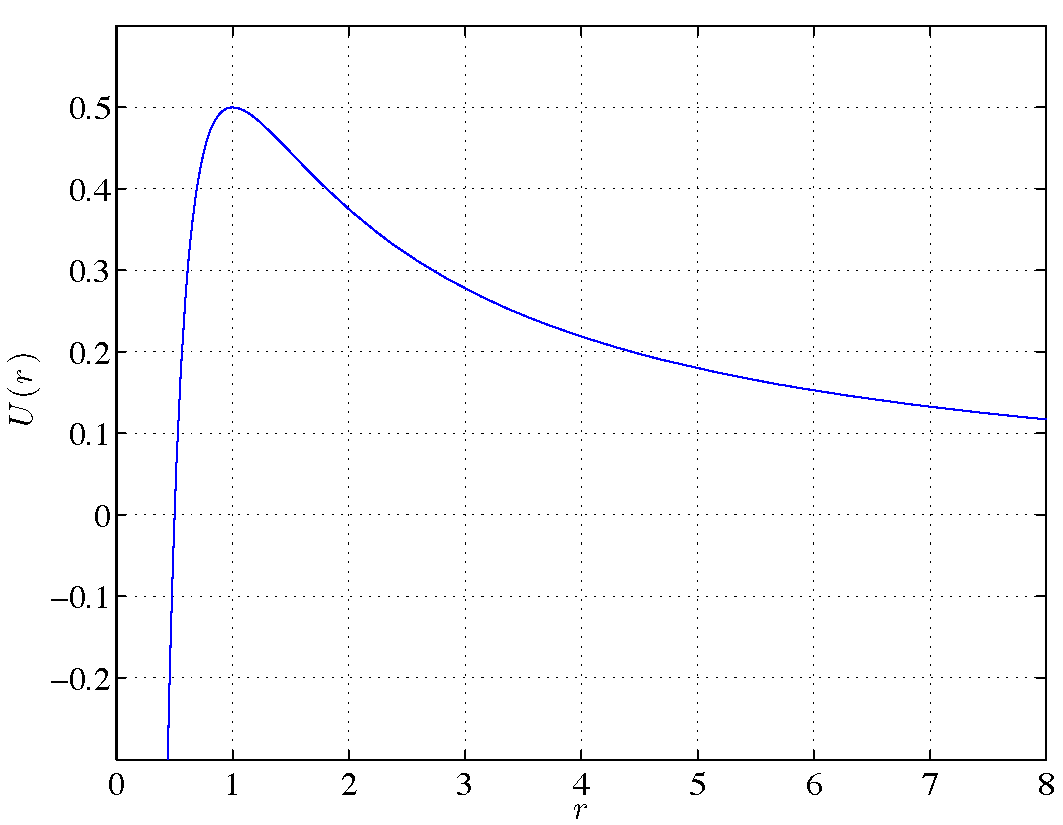
\includegraphics[width=0.45\textwidth]{probC.eps}}
%
%\noindent This graph approaches 0 from above as $r\rightarrow\infty$, and it approaches $-\infty$ as $r\rightarrow-\infty$.
%\begin{subprob}\setcounter{enumi}{1}
%\item What are the possible types of the orbit when $C>0$. 
%\vspace*{0.2cm}
%\item What are the possible types of the orbit when $C<0$. 
%\vspace*{0.2cm}
%\item What is the value of the energy constant $C$ for a circular orbit.
%\end{subprob}
%
%
%\end{prob}

\end{document}

